\section{Dataset and Split Protocol}
\label{sec:data}

\subsection{Class Definition and Split Roots}

The classifier is trained over seven strawberry health states:
\emph{drought}, \emph{frost}, \emph{gray mold}, \emph{healthy},
\emph{overwatered}, \emph{root rot}, and \emph{white mold}. The seven
classes are not pairwise visually orthogonal; in particular, the
\emph{drought}/\emph{overwatered} and \emph{overwatered}/\emph{root rot}
pairs share several mid-stage symptoms, and the two mold classes share
fruit-surface presentation. Operational definitions and primary
visual indicators are summarized in Table~\ref{tab:class-defs}; the
full per-class symptom, cause, and treatment lists are maintained in
the disease knowledge graph used by the runtime retrieval module.

\begin{table*}[t]
\centering
\caption{Operational definitions of the seven disease classes,
extracted from the runtime disease knowledge graph. The primary visual
indicator listed here is the head symptom from the corresponding
knowledge-graph entry; classes are not pairwise visually orthogonal,
which motivates the constrained dual-report policy of
\S\ref{sec:dualpolicy} for semantically plausible close pairs.}
\label{tab:class-defs}
\begin{tabular}{l l p{0.55\linewidth}}
\toprule
Class & Severity & Primary visual indicator \\
\midrule
Drought & moderate & Leaf margins curl inward and become dry, papery, and brittle. \\
Overwatered & moderate & Persistently wet or saturated growing media; standing water in the root zone. \\
Root rot & severe & Wilting during midday heat despite adequate soil moisture (water uptake failure). \\
Frost & variable & Glassy, water-soaked translucent tissue on leaves and petioles immediately after thaw. \\
Gray mold & severe & Gray, fuzzy sporulation covering fruit surfaces, flowers, or stem lesions (\emph{Botrytis cinerea}). \\
White mold & severe & Cottony white mycelium growing on stems, crown base, or fruit (\emph{Sclerotinia sclerotiorum}). \\
Healthy & none & Evenly colored dark-green foliage without spots, lesions, or discoloration. \\
\bottomrule
\end{tabular}
\end{table*}

The dataset is organized into three on-disk roots, each holding seven
class subdirectories:

\begin{itemize}[leftmargin=1.3em]
    \item the \emph{compact training} root (\texttt{train}), which stores
    the unaugmented source-image pool;
    \item the \emph{augmented training} root (\texttt{train\_aug}), the
    active classifier-training root and stage-2 generation root, derived
    from \texttt{train} via deterministic class-floor balancing;
    \item the \emph{holdout} root, a physically separate directory tree
    used for evaluation only.
\end{itemize}

Per-class counts at the time of writing are reported in
Table~\ref{tab:dataset-counts}; Figure~\ref{fig:dataset-composition}
visualizes the same counts, and Figure~\ref{fig:holdout-grid} shows
representative holdout examples.

\begin{table}[H]
\centering
\caption{Per-class image counts in the three split roots. Counts reflect the
state after the holdout release, augmented-root rebuild, class-floor
balancing, and conservative external image audit described in this section.}
\label{tab:dataset-counts}
\begin{tabular}{lrrr}
\toprule
Class & train & train\_aug & holdout \\
\midrule
Drought & 57 & 300 & 10 \\
Frost & 109 & 300 & 10 \\
Gray mold & 602 & 602 & 10 \\
Healthy & 322 & 322 & 10 \\
Overwatered & 71 & 300 & 10 \\
Root rot & 129 & 300 & 10 \\
White mold & 216 & 300 & 10 \\
\textbf{Total} & \textbf{1506} & \textbf{2424} & \textbf{70} \\
\bottomrule
\end{tabular}

\end{table}

\begin{figure}[H]
\centering
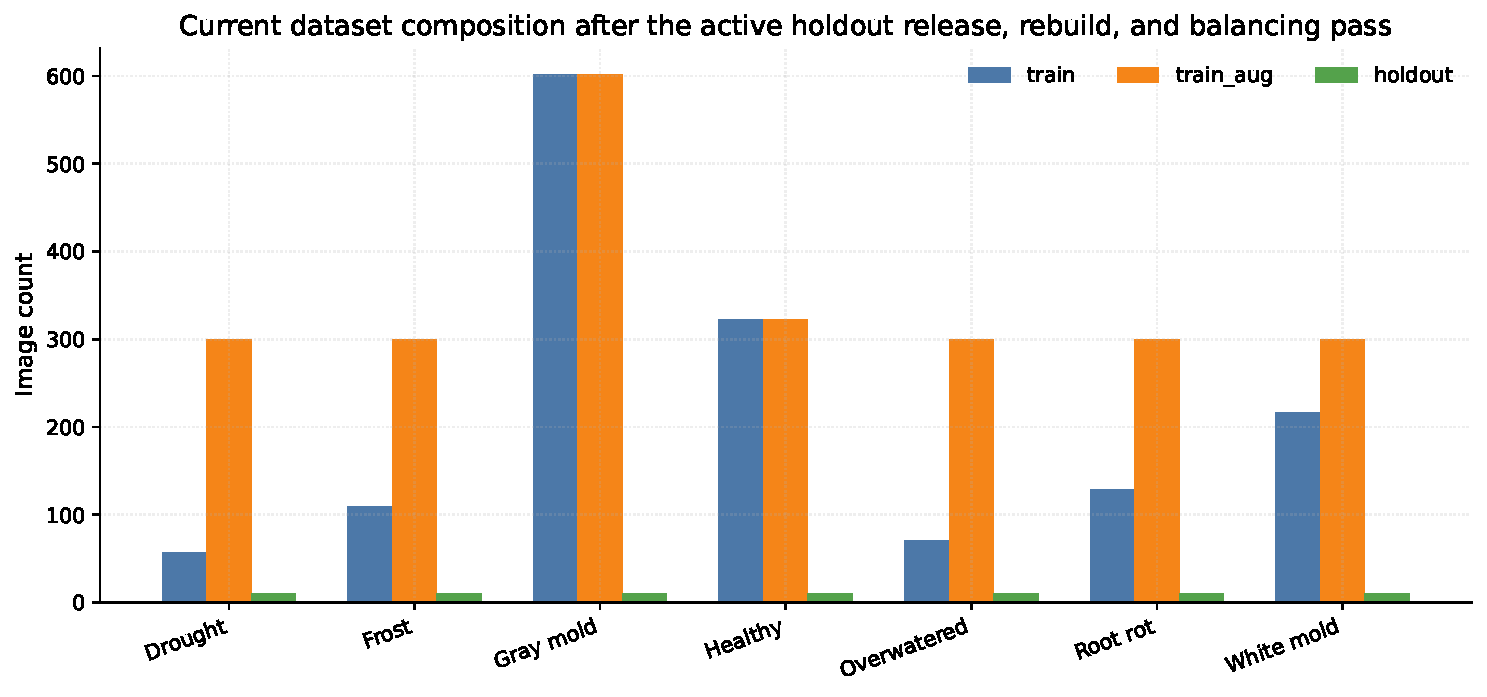
\includegraphics[width=\linewidth]{figures/generated/dataset_composition.pdf}
\caption{Per-class image counts in the compact training split, the
augmented training split, and the active balanced holdout. The augmented
split enforces a minimum of 300 images for each underrepresented class.}
\label{fig:dataset-composition}
\end{figure}

\begin{figure}[H]
\centering
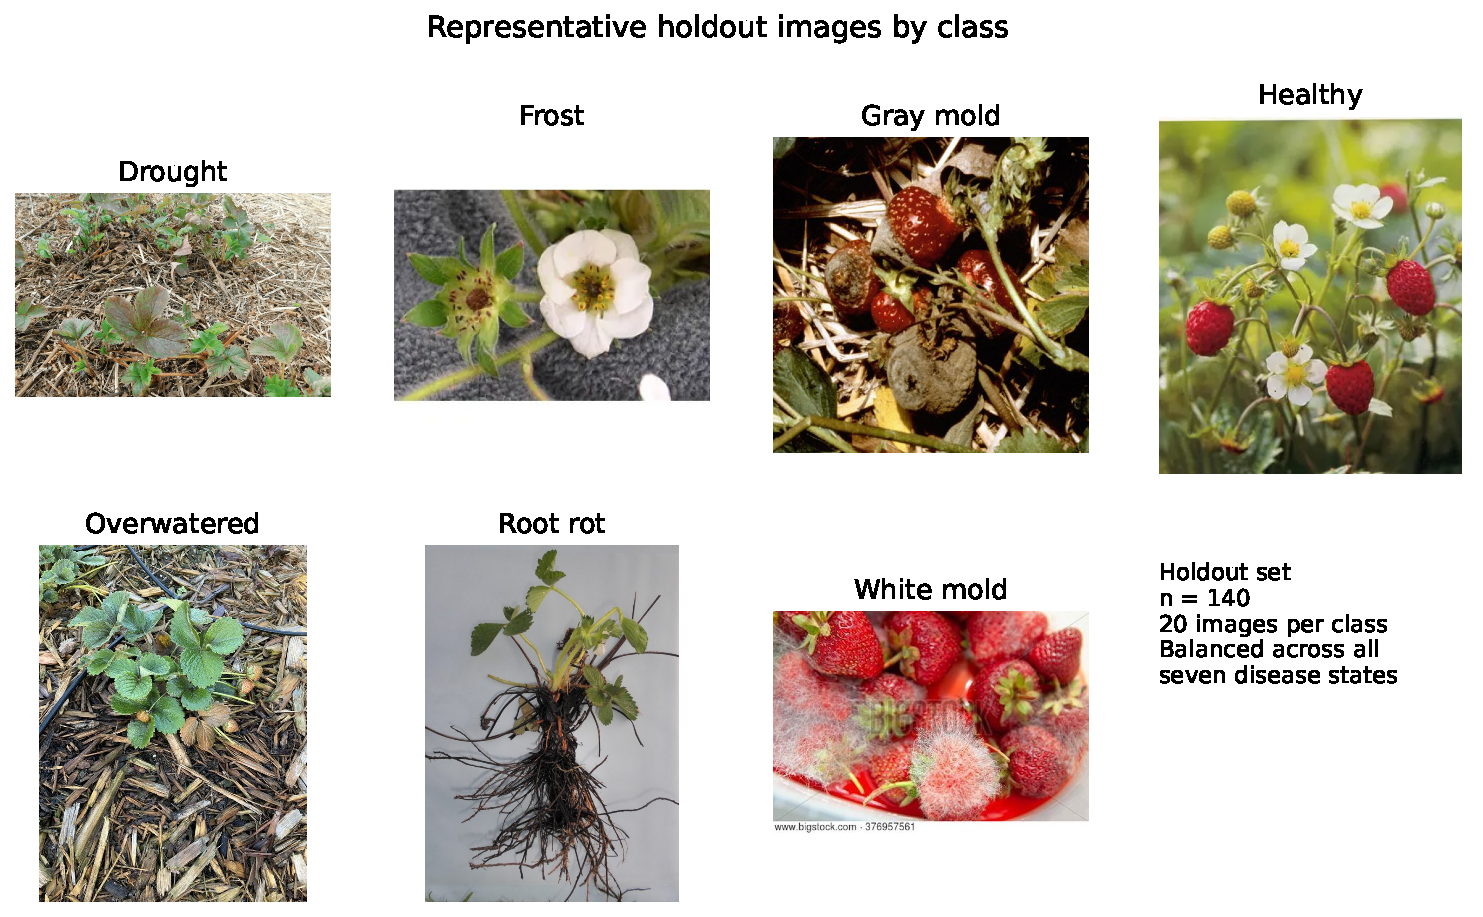
\includegraphics[width=\linewidth]{figures/generated/holdout_examples_grid.pdf}
\caption{Representative holdout images, one per class. The active holdout
contains 10 images per class for a total of $n{=}70$ evaluation images.}
\label{fig:holdout-grid}
\end{figure}

\subsection{Holdout Construction by Physical Relocation}

The active holdout was constructed by relocating source files out of the
training roots, rather than by maintaining a logical exclusion manifest.
Logical exclusion is sufficient under disciplined data loading but
silently fails when a downstream training script enumerates a directory
tree with default settings, which is a common mode in practice. Physical
relocation removes the file from the training tree entirely; a default
loader cannot re-include it.

The current holdout contains 10 images per class for a total of 70
images. For \emph{gray mold} and \emph{white mold}, the compact and
augmented training roots originally matched one-to-one, which simplified
holdout selection. For the non-mold classes, the augmented root
contained augmentation descendants whose source stems were already
present in the training pool. To prevent partial holdout representation
in training, each holdout source stem was relocated together with its
\texttt{\_augNNN} descendants.

After an earlier larger-balanced-holdout iteration, 10 images per class
were released from the holdout back into the compact training root in
order to recover support for underrepresented classes while preserving a
balanced evaluation tree. The augmented root was then rebuilt from the
compact root rather than patched in place, eliminating any silently
surviving balancing artifacts from prior states.

\subsection{Class-Floor Balancing}

The augmented training root was balanced via a deterministic class-floor
augmentation routine that raises any underrepresented class to a minimum
of 300 images. The augmentations are deliberately conservative: horizontal
flips, small-angle rotations, mild brightness or contrast perturbations,
and a flip-plus-rotation composite. This design follows the standard
recommendation that low-distortion augmentations preserve the disease
appearance in agricultural images more reliably than aggressive synthetic
transformations~\citep{shorten2019augmentation}. Classes that already
exceeded the floor are not modified.

\subsection{Conservative External-Image Audit}

In addition to the internal split work, the training state incorporates an
earlier human-audited external image audit. After review, six visually
defensible non-duplicate images were retained: five \emph{frost} and one
\emph{drought}. These images were inserted into the compact training root
and given deterministic augmentation descendants in the rebuilt augmented
root.

\subsection{Effect of the Split Protocol}

The current split state addresses two failures of prior iterations.
First, the active holdout no longer overrepresents the mold classes
relative to the non-mold classes; per-class support is uniform at 10.
Second, no holdout source stem (or any of its augmentation descendants)
remains in the training roots. Combined with the class-floor balancing,
this leaves the augmented training split with no class below the minimum
floor of 300 for previously underrepresented categories. We measure all
classifier results in \S\ref{sec:results} on this active holdout.
